
\chapter{Scala CPS plugin examples}\label{chap:cps-examples}

\begin{figure}[h!]
\begin{lstlisting}
val v1 = reset {
  shift { k: (Int=>Int) =>
    k(7)
  } + 1
} * 2
println(v1) // prints 16
\end{lstlisting}
\caption{A simple numeric example. The value of the \texttt{reset} block is equal to the value of the \texttt{shift} block plus one. The \texttt{shift}, block gets the rest of the continuation in the form of the function \texttt{k}, which in this case is the function \(x + 1\). The shift block invokes \texttt{k} with the argument 7 and returns the resulting value 8, which is then the value of the \texttt{reset} block. This value is then multiplied by 2 (outside the continuation), so the printed value is 16.}
\label{fig:example_cps_1}
\end{figure}




\begin{figure}[h!]
\begin{lstlisting}
val v2 = reset {
  shift { k: (Int=>Int) =>
    k(k(k(7)))
  } + 1
} * 2
println(v2) // prints 20
\end{lstlisting}
\caption{Example showing that the rest of the continuation may be called multiple times. In this case, the rest of the continuation is invoked three times. The final result of the continuation is multiplied by 2 outside the continuation (resulting in the value 20).}
\label{fig:example_cps_2}
\end{figure}




\begin{figure}[h!] 
\begin{lstlisting}
val result = reset {
  println("entering first shift")
  val firstShift = shift { k: (Int => Int) =>
      val res = k(0)
      println(s"exiting first shift, res = $res")
      res
  } + 1

  println(s"firstShift = $firstShift; entering second shift")
  val secondShift = shift { k: (Int => Int) =>
      val res: Int = k(firstShift)
      println(s"exiting second shift, res = $res")
      res
  } + 1
  println(s"secondShift = $secondShift; returning the reset")

  secondShift
}

println(s"result = $result")

// entering first shift
// firstShift = 1; entering second shift
// secondShift = 2; returning the reset
// exiting second shift, res = 2
// exiting first shift, res = 2
// result = 2
\end{lstlisting}
\caption{Example showing the control flow throughout the reset block when there is more than one shift block. Notice the similarity with multiple function calls.}
\label{fig:example_cps_step_by_step}
\end{figure}



\begin{figure}[h!] 
\begin{lstlisting}
import scala.util.continuations._

object TwelveDaysOfChristmas extends App {
  val daysAndGifts = Seq(
    ("First", "a Patridge in a Pear Tree"),
    ("Second", "Two Turtle Doves"),
    ("Third", "Three French Hens")
  )
  val days = daysAndGifts.map(_._1)
  val gifts = daysAndGifts.map(_._2)

  val carol: List[String] = reset {
    val dayIndex: Int = shift {
      verse: (Int => List[String]) =>
        (0 to days.length - 1).foldRight(List.empty[String])((day, list) => "" :: verse(day) ::: list)
    }

    // the continuation below this line calculated a single verse for the day identified by `dayIndex`
    val dayLine = s"On the ${days(dayIndex)} day of Christmas my true love sent to me"
    val giftIndex: Int = shift {
      line: (Int => String) =>
        dayLine :: (0 to dayIndex).foldLeft(List.empty[String])((list, gift) => line(gift) :: list)
    }

    // the continuation below this line calculates a single line of a verse, the line identified by `giftIndex`

    val gift = gifts(giftIndex)
    val line = if (dayIndex == 0) {
      s"$gift."
    } else if (giftIndex > 0) {
      s"$gift,"
    } else {
      s"and $gift."
    }
    line
  }
  carol.foreach(println(_))

  /*
  On the First day of Christmas my true love sent to me
  a Patridge in a Pear Tree.

  On the Second day of Christmas my true love sent to me
  Two Turtle Doves,
  and a Patridge in a Pear Tree.

  On the Third day of Christmas my true love sent to me
  Three French Hens,
  Two Turtle Doves,
  and a Patridge in a Pear Tree.  */
}
\end{lstlisting}
\caption{An example printing the first three verses of the well-known Christmas carol ``The Twelve Days of Christmas''. Notice the answer type modification.}
\label{fig:example_twelve_days}
\end{figure}






\begin{figure}

    \begin{minipage}{.7\linewidth}
      \centering
        \begin{lstlisting}
import scala.util.continuations._
import scala.swing._

object ContinuationsSwingApp extends SimpleSwingApplication {

  var continue: (Unit => Unit) = { _ => run()}

  def run() {
    reset {
      val first = ask("What is your first name?")
      val last = ask("What is your last name?")
      label.text = s"Hello, $first $last!"
    }
  }

  def ask(prompt: String): String@cpsParam[Unit, Unit] = {
    label.text = prompt
    shift {
      k: (Unit => Unit) => {
        continue = k
      }
    }
    textField.text
  }

  val textField = new TextArea(10, 40)
  val label = new Label("Welcome to the demo app")
  val button = new Button(new Action("Next") {
    override def apply(): Unit = continue()
  })

  override def top: swing.Frame = new MainFrame {
    contents = new BorderPanel {
      add(label, BorderPanel.Position.North)
      add(textField, BorderPanel.Position.Center)
      add(button, BorderPanel.Position.South)
    }
  }
}
\end{lstlisting}
    \end{minipage}%
    \begin{minipage}{.3\linewidth}
      \centering

        \begin{tabular}{c}
Step1:\\
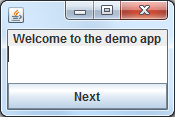
\includegraphics[width=0.9\linewidth]{images/swing-demo-step1.png} \\[0.7cm] 
Step2:\\
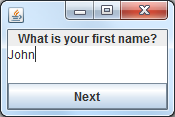
\includegraphics[width=0.9\linewidth]{images/swing-demo-step2.png} \\[0.7cm]
Step3:\\
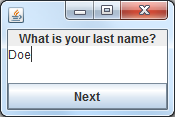
\includegraphics[width=0.9\linewidth]{images/swing-demo-step3.png} \\[0.7cm]
Step4:\\
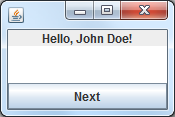
\includegraphics[width=0.9\linewidth]{images/swing-demo-step4.png} \\
\end{tabular}

    \end{minipage} 


\caption{A simple Swing application with an event-based control flow defined in imperative style (see method \texttt{run}). For each question, the flow is suspended and the \texttt{shift} blocks assigns the rest of the continuation to a variable. Pushing the button resumes the continuation.}
\label{fig:example_shift-reset-swing}
\end{figure}





\chapter{Scala.React examples}\label{chap:scala-react-examples}



\begin{figure}[h!] 
\begin{lstlisting}
object person {
  val firstName = Var("John")
  val lastName = Var("Doe")
  val fullName = Strict { firstName() + " " + lastName() }
}

observe(person.firstName) {
  firstName =>
    println(s"The first name changed to $firstName, and last name is ${person.lastName.now}.")
}

observe(person.lastName) {
  lastName =>
    println(s"The last name changed to $lastName, and the first name is ${person.firstName.now}.")
}

observe(person.fullName) {
  fullName =>
    println(s"Full name changed to $fullName.")
}

def changeName() {          
  person.firstName() = "Jane"
  person.lastName() = "Roe"
}
// calling `changeName' prints the following:
//
// The first name changed to Jane, and last name is Roe.
// The last name changed to Roe, and the first name is Jane.
// Full name changed to Jane Roe.
\end{lstlisting}
\caption{This example demonstrates that observers always see the state of the application in a consistent state. With using traditional observer pattern, the observers would see the person having the name ``Jane Doe'' before it finally changes to ``Jane Roe''.}
\label{fig:example_scala-react-consistency}
\end{figure}





\begin{figure}[h!] 
\begin{lstlisting}
object MyDomain extends Domain {
  val scheduler = new SwingScheduler()
  val engine = new Engine
} import MyDomain._

object ScalaReactLineDrawing extends SimpleSwingApplication with Observing{
  override def main(args: Array[String]) {
    schedule { startup(args) }
    start() // starts the scala-react engine
  }
  override def top: Frame = new MainFrame() {
    contents = new FlowPanel() {
      val mouseDown = EventSource[Point]
      val mouseMove = EventSource[Point]
      val mouseUp = EventSource[Point]

      val mainProgramFlow = Reactor.loop {
        self =>
        // step 1
          val path = new Path(self await mouseDown)
          self.loopUntil(mouseUp) {
            // step 2
            val m = self awaitNext mouseMove
            path.lineTo(m)
            draw(path)
          }
          path.close() // step 3
          draw(path)
      }

      listenTo(mouse.clicks, mouse.moves) // scala.swing events
      reactions += {
        case MousePressed(_, point, _, _, _) => mouseDown << point
        case MouseReleased(_, point, _, _, _) => mouseUp << point
        case MouseDragged(_, point, _) => mouseMove << point
      }
      class Path(var positions: Seq[Point]) {
        def this(pos: Point) = this(Seq(pos))
        def lineTo(pos: Point) { positions = positions :+ pos }
        def close() { positions = positions :+ positions.head }
      }
      var pathDrawn = new Path(new Point(0, 0))
      def draw(path: Path) { pathDrawn = path; repaint() }
      override protected def paintComponent(g: swing.Graphics2D): Unit = {
        super.paintComponent(g)
        val xPoints = pathDrawn.positions.map(pos => pos.x).toArray
        val yPoints = pathDrawn.positions.map(pos => pos.y).toArray
        g.setColor(Color.BLACK)
        g.drawPolyline(xPoints, yPoints, pathDrawn.positions.length)
} } } }
\end{lstlisting}
\caption{A sample application painting a closed line with the mouse using Scala.React \emph{reactor} and \emph{event streams}.}
\label{fig:example_scala-react-line-drawing}
\end{figure}










